% Upper contours are qualitative; lower panels retain exact analytic data at native width.
% Volume three architecture figures. Independent export only; not book fonts.
\colorlet{MutedBlueFill}{FigureBlueFill}
\colorlet{MutedGreenFill}{FigureGreenFill}
\colorlet{MutedPurple}{FigurePurple}
\colorlet{MutedPurpleFill}{FigurePurpleFill}
\tikzset{
 v3 picture/.style={x=1mm,y=1mm,font=\figurefont\fontsize{8}{10}\selectfont,text=FigureInk,line width=.65pt},
 v3 box/.style={draw=FigureBlue,fill=white,rounded corners=1.8pt,line width=.7pt,inner sep=2.5pt,align=center},
 v3 data/.style={v3 box,fill=FigureBlueFill},
 v3 model/.style={v3 box,draw=FigureGreen,fill=FigureGreenFill},
 v3 output/.style={v3 box,draw=FigureYellow,fill=FigureYellowFill},
 v3 risk/.style={v3 box,draw=FigureRed,fill=FigureRedFill},
 v3 group/.style={draw=FigureBlue,rounded corners=1.8pt,line width=.65pt,inner sep=3mm},
 v3 flow/.style={draw=FigureStroke,line width=.75pt,-{Stealth[length=1.65mm,width=1.05mm]},rounded corners=1pt},
 v3 guide/.style={draw=FigureMuted,line width=.6pt,dashed},
 v3 feedback/.style={v3 flow,draw=FigureGreen,dashed},
 v3 title/.style={draw=none,fill=none,font=\figurefont\fontsize{8}{10}\selectfont,align=center,inner sep=1pt},
 v3 note/.style={draw=none,fill=none,font=\FigureNoteFont\fontsize{7.5}{9.5}\selectfont,text=FigureMuted,align=center,inner sep=1pt},
 v3 label/.style={draw=none,fill=none,font=\figurefont\fontsize{8}{10}\selectfont,align=center,inner sep=1pt},
 v3 wire/.style={draw=FigureMuted,line width=.45pt},
 v3 point/.style={circle,draw=FigureBlue,fill=FigureBlueFill,minimum size=2.3mm,inner sep=0pt,line width=.55pt}
}
% Bring pre-existing native TikZ geometry to the same typography and scale.
\tikzset{
 foundation picture/.append style={font=\figurefont\fontsize{8}{10}\selectfont,line width=.65pt},
 foundation node/.append style={rounded corners=1.8pt,line width=.7pt,font=\figurefont\fontsize{8}{10}\selectfont},
 foundation heading/.append style={draw=none,fill=none,font=\figurefont\fontsize{8}{10}\selectfont},
 foundation note/.append style={draw=none,fill=none,font=\FigureNoteFont\fontsize{7.5}{9.5}\selectfont},
 foundation flow/.append style={line width=.75pt,-{Stealth[length=1.65mm,width=1.05mm]}},
 foundation frame/.append style={rounded corners=1.8pt,line width=.7pt},
 foundation edge label/.append style={draw=none,fill=none,font=\figurefont\fontsize{8}{10}\selectfont}
}
% Official Lucide outline icons, consistently used across diagrams. Size in mm.
\newcommand{\VIcon}[5]{\node[inner sep=0pt] at (#2,#3) {\includegraphics[width=#4mm]{figures/03-foundations/00-shared/tikz/icons/#1-#5.pdf}};}
% A neutral network glyph (not a claim about an actual model architecture).
% Coordinates denote its centre; scale 1 gives 13 x 8 mm.
\newcommand{\VNet}[4]{\begin{scope}[shift={(#1,#2)},scale=#3]
 \foreach \a in {-3,0,3}{\foreach \b in {-3,0,3}{\draw[v3 wire] (-5,\a)--(0,\b);}}
 \foreach \a in {-3,0,3}{\draw[v3 wire] (0,\a)--(5,0);}
 \foreach \a in {-3,0,3}{\draw[draw=#4,fill=#4,line width=.55pt] (-5,\a) circle(.9);\draw[draw=#4,fill=white,line width=.55pt] (0,\a) circle(.9);}
 \draw[draw=#4,fill=#4,line width=.55pt] (5,0) circle(.9);
\end{scope}}
\newcommand{\VDots}[4]{\foreach \k in {0,1,2,3}{\fill[#4] ({#1+2.7*\k},#2) circle(#3);}}
% Feature vector/tensor elements are scientific glyphs, not decorative icons.
\newcommand{\VVector}[4]{\foreach \k in {0,...,4}{\fill[#4,rounded corners=.25pt] ({#1+2.2*\k},#2) rectangle ++(1.5,#3);}}

\colorlet{VNetworkInput}{FigureBlue}\colorlet{VNetworkHidden}{FigureYellow}\colorlet{VNetworkOutput}{FigureGreen}
\begin{tikzpicture}[v3 picture]
\tikzset{v3 box/.append style={line width=.8pt},v3 group/.append style={line width=.85pt},v3 flow/.append style={line width=.9pt}}
\path[use as bounding box] (0,0) rectangle (163,118);
\node[v3 title,text=FigureBlue] at (39,114) {窄谷（尖锐）};
\node[v3 title,text=FigureGreen] at (123,114) {宽谷（平坦）};
% Compact level-set glyphs; labels remain 8pt, with no overall scale change.
\foreach \rx/\ry in {7/14.875,5.25/11.375,3.5/7.875,1.75/4.375}{\draw[FigureBlue,fill=FigureBlueFill,line width=.75pt] (38,96.5) ellipse ({\rx} and {\ry});}
\foreach \rx/\ry in {30/14.5,25/11.5,19/8.55,13/5.6,7/2.6}{\draw[FigureGreen,fill=FigureGreenFill,line width=.75pt] (123,96.5) ellipse ({\rx} and {\ry});}
\foreach \x/\c in {38/FigureBlue,123/FigureGreen}{
 \fill[\c] (\x,96.5) circle(.9);
 \draw[v3 flow,draw=\c] (\x,96.5)--({\x+4},101.5);
 \draw[draw=\c,fill=white,line width=.8pt] ({\x+4},101.5) circle(1.1);
}
\draw[v3 flow,dashed,draw=FigureBlue] (38,95)--(38,80)--(28,80)--(28,78);
\draw[v3 flow,dashed,draw=FigureGreen] (123,95)--(123,80)--(112,80)--(112,78);
% Parameter perturbation -> complete predictor -> loss, for both local geometries.
\foreach \x/\c/\fc in {28/FigureBlue/FigureBlueFill,112/FigureGreen/FigureGreenFill}{
 \draw[draw=\c,fill=\fc,dashed] (\x,72) ellipse (10 and 6);
 \foreach \dx/\dy in {-6/-1,-4/3,-1/0,2/4,5/1,3/-3,-4/-3}{\fill[\c] ({\x+\dx},{72+\dy}) circle(.65);}
 \node[v3 box,draw=\c,minimum width=18mm,minimum height=14mm] (net\x) at ({\x+24},72) {};
 \VLayerNet{\x+24}{72}{.9}{3}{4}{1}
 \draw[v3 flow,draw=\c] ({\x+10},72)--(net\x.west);
 \draw[v3 flow,draw=\c] (net\x.east)--({\x+36},72);
 \node[v3 label] at ({\x+43},72) {损失};
 \node[v3 label,anchor=north] at (\x,64) {参数扰动};
 \node[v3 label,anchor=north] at ({\x+24},64) {预测器};
 \node[v3 label,text=\c] at ({\x+9},57.5) {扰动平均损失 $\hat R_S(Q)$};
}
% The two posterior risks still require the PAC-Bayes prior cost.
\draw[v3 flow,draw=FigureBlue] (55,57.5)--(63,57.5);
\draw[v3 flow,draw=FigureGreen] (103,57.5)--(98,57.5);
\VIcon{scale}{69}{57.5}{6}{purple}
\node[v3 label,anchor=west] at (75,59) {泛化保证};
\node[v3 note,anchor=west] at (75,55) {还需先验代价};
% Exact 0.1+0.45*s^2 and 0.1+0.08*s^2, unchanged source and 163mm width.
\node[inner sep=0pt,anchor=south west] at (0,0) {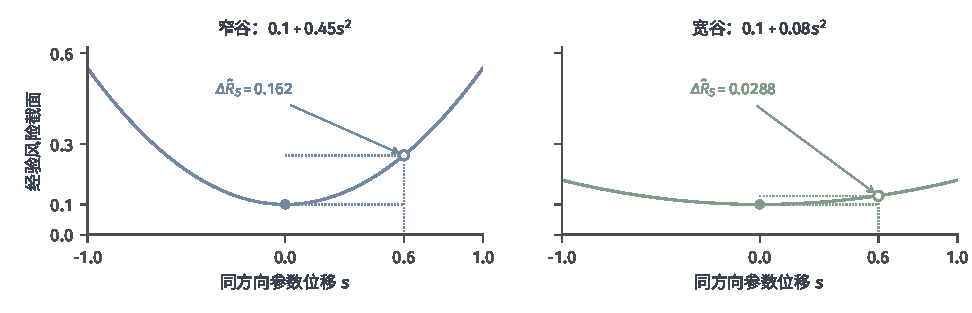
\includegraphics[width=163mm]{figures/03-foundations/02-learning-theory/generated/learning-theory-flat-sharp/quantitative-panels.pdf}};
\end{tikzpicture}
